% choose the document class
% use scrreport for big documents with chapters
% use scrartcl for smaller documents with only sections
\documentclass[
    pdftex,                % compiler
    oneside,               % onesided printing, e.g. relevant for binding correction
	11pt,                  % fontsize
	parskip=half,          % Space (in lines) between paragraphs	
	headheight = 12pt,     % Header hight
	headsepline,           % Line after header
	footheight = 16pt,     % Footer height
	footsepline,           % Line before footer
	abstract=true,         % Abstract headline
	DIV=calc,              % Calculate print space
	BCOR=8mm,              % binding correction setting (shift to the left to account for space occupied by binding)
	headinclude=false,     % Exclude header from print space
	footinclude=false,     % Exclude footer from print space
	listof=totoc,          % Show List of Figures/Tables in Contents
	toc=bibliography,      % Show Bibliography in Contents
]{scrreport}

% import the template-packages
\usepackage{structure/text-options}
\usepackage{structure/code-listings}
\usepackage{structure/float-objects}
\usepackage{structure/extended-glossary}
\usepackage{structure/bibliography}

% Now the document structure. Feel free to comment out sections you don't need.
\begin{document}
    % Initialize document
    \defineColors{}
    \RedeclareSectionCommand[beforeskip=\chapterMargin]{chapter}
    \include{content/glossary}
    
    % The Titlepage
    \def\titletext{Fichtenweg 17 U}

\begin{titlepage}
    % If you have a fitting Title-Logo put it here instead of the vertical space.
    % But be careful, the uni Tübingen e.g. EXPLICITLY PROHIBITS the use of their logo!!!
    % see for details:
    % https://uni-tuebingen.de/fakultaeten/wirtschafts-und-sozialwissenschaftliche-fakultaet/faecher/fachbereich-sozialwissenschaften/sportwissenschaft/studium/abschlussarbeit-studienende/faq-abschlussarbeit/#c1657287
    %\begin{center}
	%    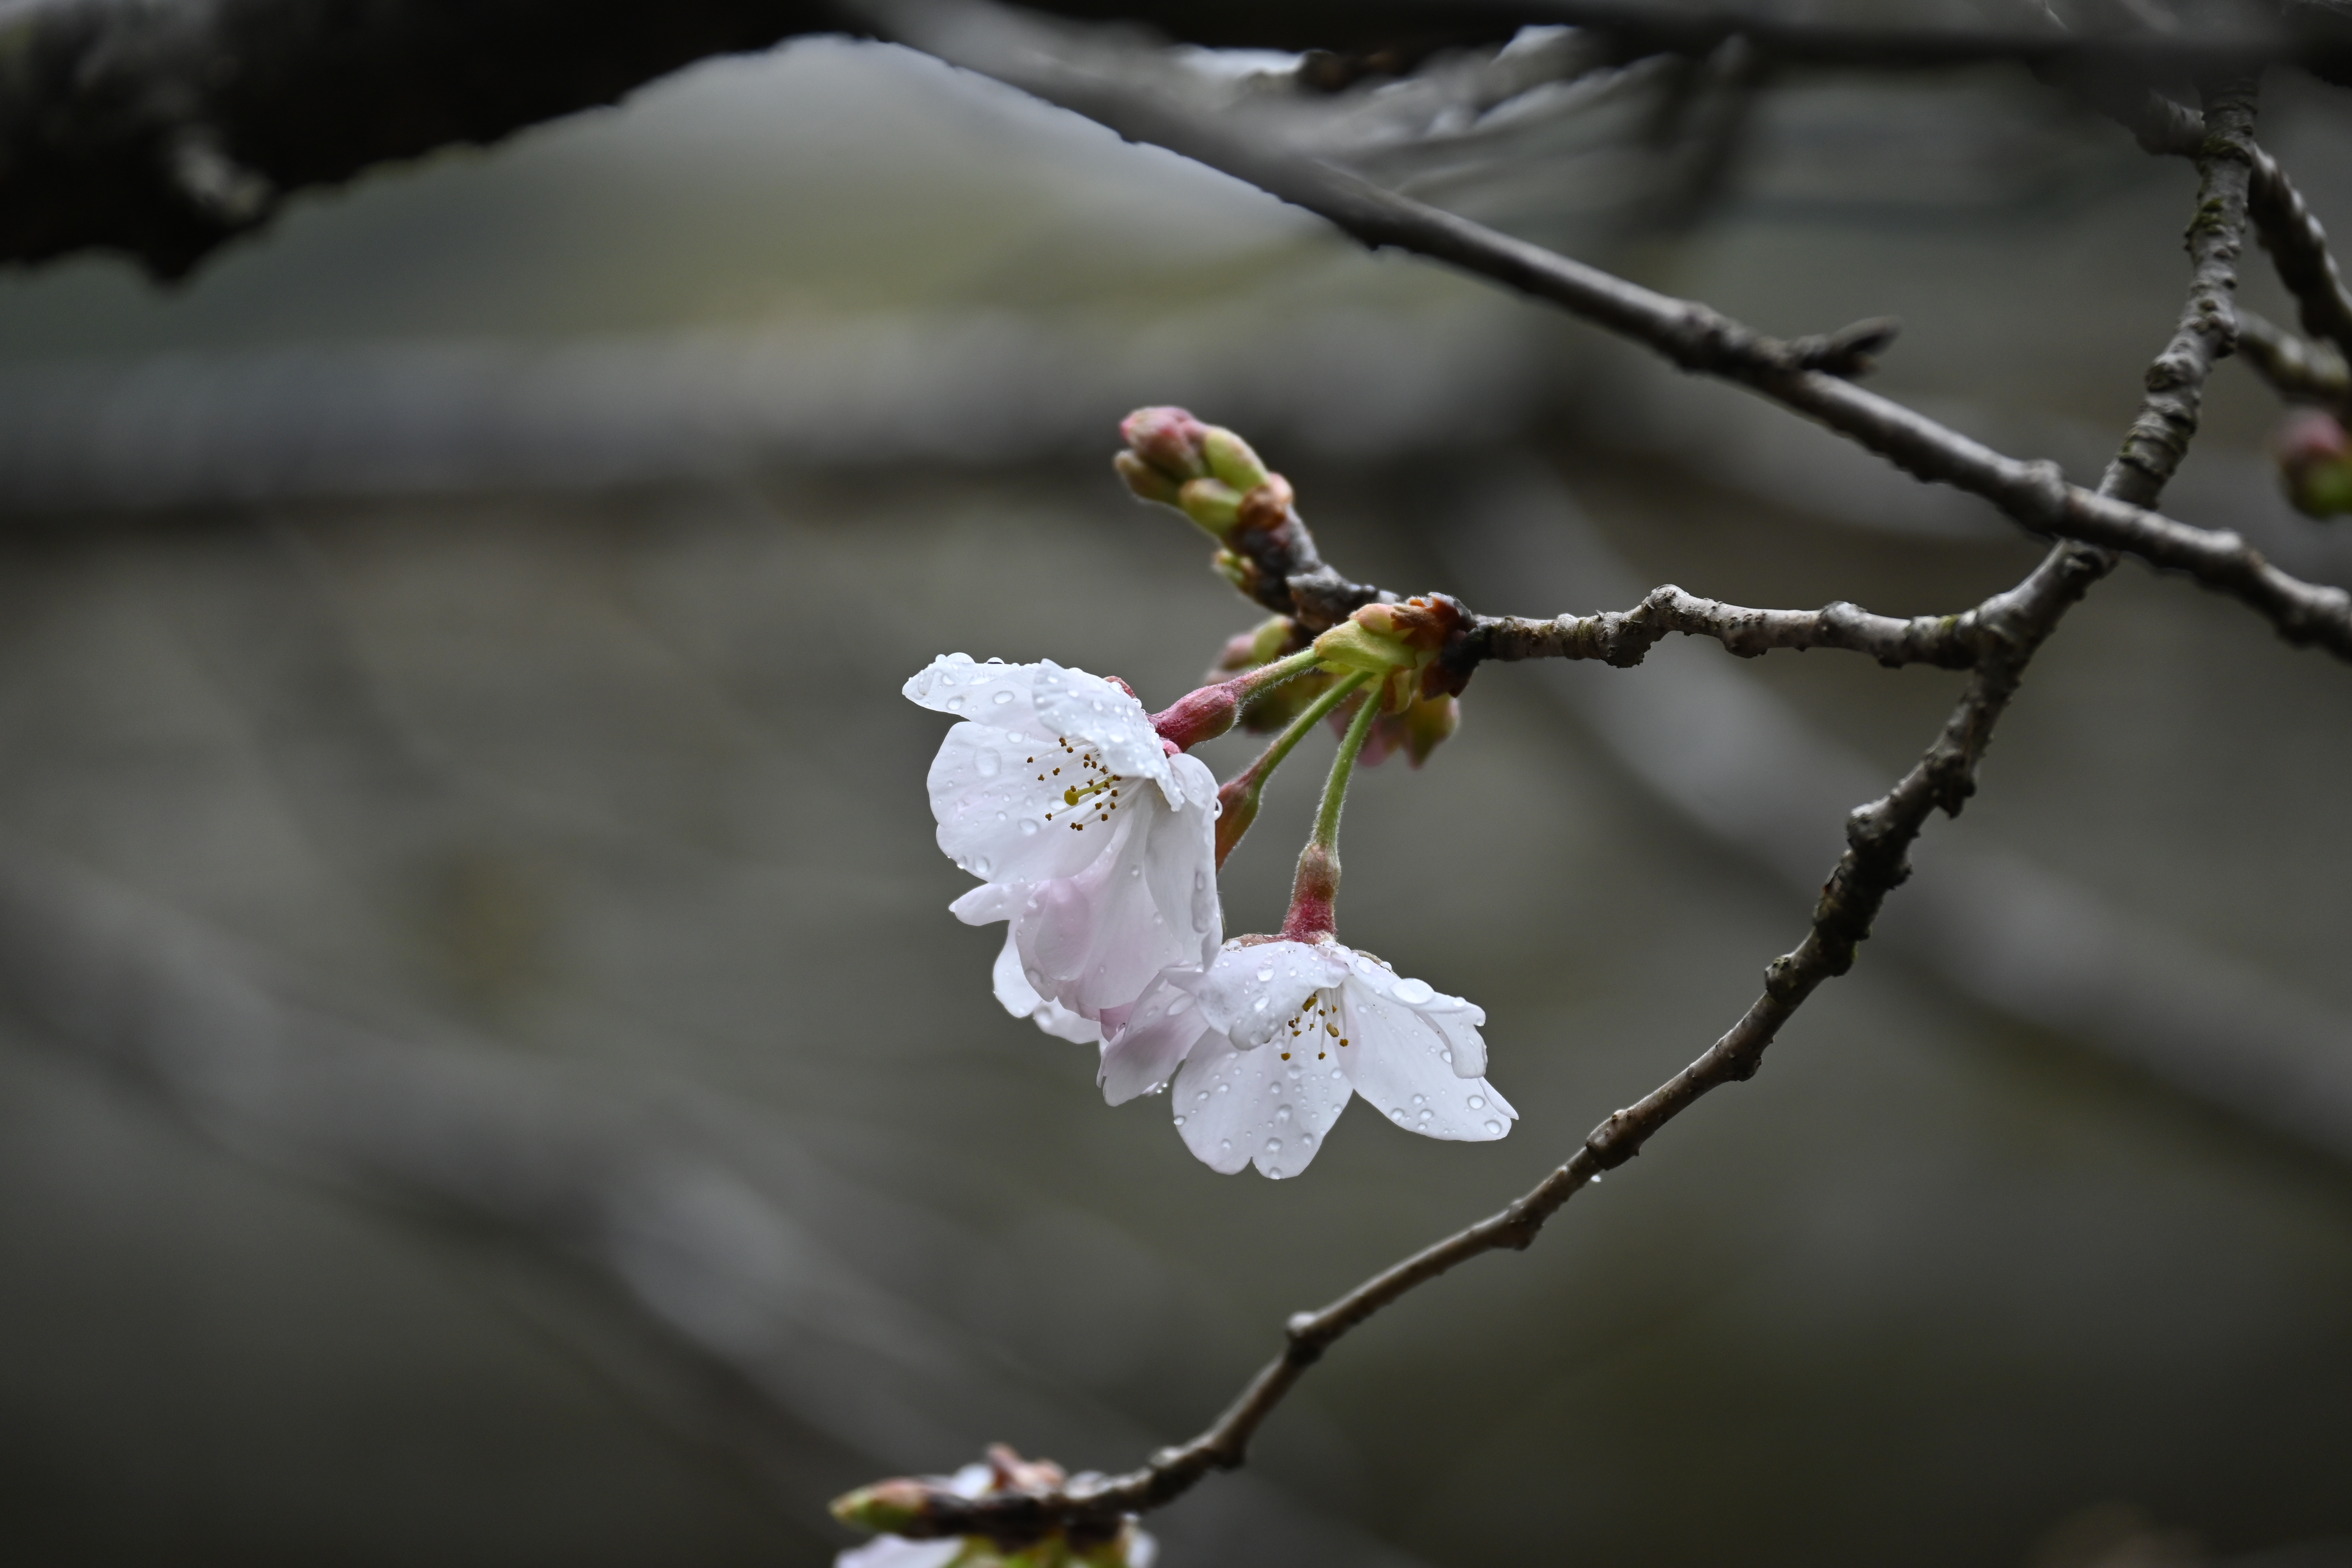
\includegraphics[height=2.5cm] {images/example-image.jpg}
	%\end{center}
    \vspace*{3cm}

    % Title, subtitle, etc.
	\begin{center}
    	\doublespacing{
    		\vspace*{12mm}
            Welcome!\\
            to our\\
            
    		\vspace*{6mm}
            {\LARGE\textbf {\titletext}}\\
            
    		\vspace*{6mm}
            Community Guidelines\\
    	}
	\end{center}
 
	% Push the table to the bottom of the page.
	\enlargethispage{20mm}
	\vfill

	\begin{center}
        \textbf{Version}: \today
	\end{center}
 
\end{titlepage}
\newpage

    % Start with roman numbering for declaration and abstract
    \pagenumbering{Roman}
    \pagestyle{empty}

% override abstract headline
\renewcommand{\abstractname}{What's this about?}

\begin{abstract}

Hey there!

If you are a visitor and searching for WiFi, the kitchen is the place you are looking for! You will find a QR code on the back by the speakers that should cover your needs. And don't worry, I'll not be mad if you skip the rest of this document ;).\\
If you are or want to become a part of our floor-community: This document is for you!

First of all, Thank you for checking out our community handbook! Communication is the most important ingredient in a harmonizing community, and you have just made the first step!

Don't worry, this is not a page-long contract you need to sign with blood and sell your soul to the devil. Quite the contrary, actually! We are trying to build and maintain an open and respectful community with one primary rule:

\begin{displayquote}
    Just talk! :)
\end{displayquote}

Everyone is encouraged to speak their mind, bring new ideas, raise complaints, or just chat and have fun! Of course, in return, you are asked to have an open ear for others and respect their wishes.

Unfortunately, every community needs some place to dump all the organizational context, so this document is for that: a place to look up whom to ask, what to do, or where to go for your needs!

\end{abstract}
\newpage
     
    % Only page number in footer for directories
    \pagestyle{plain}
    % Table of contents
\begin{spacing}{1.1}
    \begingroup	
        % set subchapter depth
        \setcounter{tocdepth}{2}
        \tableofcontents
        \clearpage
    \endgroup
\end{spacing}
\newpage
    \cleardoublepage

    % Switch to document pagestyle
    \pagenumbering{arabic}
    \pagestyle{headings}

    % Chapters
    \chapter{I just arrived, what now?}

So you have just wandered into your new home for the first time and try to figure out what organizational steps you need to take to start your life here? Don't worry, we've all been there. And while the following list may not be comprehensive for you, this \quotes{Quickstart} can hopefully give you a starting point.

\section{I got keys, what are they for?}

You should have one key with teeth only on one side. That one is for the buildings main door and your room at the same time. Your room does not lock behind you automatically, but the front door will (except if a little switch is toggled), so don't forget them!

The other key with teeth on both sides is for your mail. You can find the mail room in the center of the WHO right next to the club \quotes{Kuckuck}. It is open during day hours and you should regularily check your mail. Have a look at section \ref{sec:qna-mail} for details.

All neighbors on one floor share one kitchen. As you can read in some later chapters, we decided to make the kitchen into a living space where we can meet and spend some time together. Just come and say hi whenever you like :). The washing machine is also on our floor, in the room at the bottom of the staircase, but is shared across the entire building. For details have a look at chapter \ref{sec:qna-washing-machine}.

\section{How do I register my residence?}

In Germany you are obligated to register in the city you are residing in, even if it is just for a few months. When you got the keys from the caretaker, you should have also received a letter. This \quotes{Wohnungsgeberbestätigung} is a confirmation, that you are renting a room here in WHO. With this letter you need to register at the \quotes{Bürgeramt}. As with every government-institution, it is of no use going there without an appointment, and the next free appointment might be a few weeks from now. But don't worry: You are obligated to register within the first couple of weeks of getting here, but it is enough if you schedule the appointment within that timespan, noone can blame you for having to wait for a free timeslot.

You can schedule an appointment \href{https://www.tuebingen.de/verwaltung/onlinedienste#/anmeldung_wohnsitz}{$\rightarrow{}$ here}. If you don't speak german and need help with the site, ask in chat, we are happy to help!

You can register your room as a secondary residence, but Tübingen will ask a yearly secondary-residence-tax of you if you do so. At the time of writing, this tax is ten percent of your yearly rent. You can find the details \href{https://www.tuebingen.de/verwaltung/uploads/zweitwohnungsteuersatzung.pdf}{$\rightarrow{}$ here}, though be aware that the linked PDF might not stay up to date!

\section{What the hell is the \quotes{Rundfunkbeitrag}?}

In germany we have a special tax, that finances public media like radio, public TV channels and more. It is payed per household, it does not matter if you plan on using it or not, and it is also obligatory when you are not a german citicen and only here for studying. There are special rules for flat-sharing communities, but unfortunately our dorm does not qualify for these, because we all have independently locked rooms. So yes, you need to pay the \quotes{Rundfunkbeitrag}. They will send you a letter eventually after they receive notice of your registration in Tübingen, but if you want to get it done early, you can register on \href{https://www.rundfunkbeitrag.de/buergerinnen_und_buerger/formulare/anmelden/index_ger.html}{$\rightarrow{}$ this site}. You will not safe any money, no matter when you register, they know exactly in what month you registered. As mentioned before, if you need help with the german site, just let us know.

\section{What about Uni?}

Since every study program is organized slightly different, we can't give you some globally applicable advice on how to register for courses etc. You will receive an account at some point and you will need to engage with the very user friendly tool (*not*) \href{https://alma.uni-tuebingen.de}{$\rightarrow{}$ Alma} sooner or later. For the specifics just talk to us and/or look out for introduction events for newbies at the Uni Tübingen. There are some formal ones like an introduction to alma, some events specifically for foreign students and lots of events individually organized by your \quotes{Fachschaft} (student body of your faculty). So keep an eye out for those!

One thing we can say for sure, is that you will need your student ID card as payment method for the washing machine. If you have not recieved it yet or haven't had a chance to top it up with money, contact us and we can help you out :)

\section{What recurring obligations do I need to be aware of?}

For living in WHO and studying in Tübingen you need to do the following two things every semester:

\begin{itemize}
    \item Pay the semester fee once you get notified via mail, to confirm that you want to keep studying. You can look up the details of due and completed payments in Alma > My Studies > Student Service in the tab \quotes{Payments}.
    \item Prove to the \quotes{Studierendenwerk} that you are still studying and therefore entitled to keep your room by uploading your \quotes{Immatrikulationsbescheinigung} for the next semester \href{https://tl1.eu/SWTUE/#maintenance/upload}{$\rightarrow{}$ here}. You can find the PDF in Alma > My Studies > Student Service in the tab \quotes{Requested Reports / Reports}.
\end{itemize}

\section{That's a lot, is it all set and done now?}

Well, you should definetely check for your specific case what you need to do. There is help for foreign students, talk to us or other students you know or research on your own. But I hope we were able to give you advice on the most important first steps.

And don't forget to cancel and de-register everything before you leave! You wouldn't want to pay unnecessary fees, right?
    \chapter{The folks around} \label{chap:introductions}
\newcounter{Birthdate}%
\newcounter{CurrentDate}%
\setmydatenumber{CurrentDate}{\the\year}{\the\month}{\the\day}%

Hey, you made it to the chapters! Let's start by introducing ourselves, shall we?

\section{Room U13: Robin Epple} \label{sec:robinE}
\setmydatenumber{Birthdate}{2001}{03}{31}%
\FPsub\result{\theCurrentDate}{\theBirthdate}
\FPdiv\myage{\result}{365.2425}
\FPtrunc\myage{\myage}{0}

Hi, my name is Robin and I'm \myage{} years old. I am currently in my computer science master and work as a web developer besides that. I am only partially living in Tübingen, since my hometown is closer to my office, so between the semesters I usually move there. But during the lecture time I am sure we'll run into each other at some point!

If you're looking for me, start in the kitchen ;). I love to cook for dinner and always appreciate some company, so if you're interested in joining some day, just react to my announcements in chat! Other than cooking, I love listening to epic music, I am a very passionate BeatSaber player and I have probably watched the \quotes{How to train your dragon} movies a few times too often \^{}\^{}.

Oh, and one more thing: In my bachelors I lived in a flat by myself, that's why I came here with a lot of household equipment. So if you are in need of something like a screwdriver or a vacuum, feel free to ask, maybe I can help!

I'm looking forward to meeting you!
    \chapter{The dorm-life} \label{chap:activities}

In this chapter we want to give you a quick overview on what we do as a community and how you can participate!

\section{It's cooking time!} \label{sec:cooking}
Let's start with our most important way of staying in contact: Chatting around dinner time! You will regularily find people announcing in chat, what they will be cooking and when. For most evenings this is more tailored towards small groups of three or four, but there are also bigger events once in a while where eight to nine people come together. These messages are meant as an open invitation, and everyone is welcome to join in. Whether you want to help with the preparations, just come by for eating or invite to a dinner yourself: Welcome, to our little cooking group!

Due to different schedules, preferences and wake rythms the size and constellation of people changes daily, and sometimes we also just stumble into each other while independently preparing our meals. But that just makes the conversations more interesting ;). 

If you have intolerances, ethical restrictions or just certain preferences on food, please don't let that keep you from engaging with us! Though it might not be possible to respect all wishes at all times, we will certainly do our best to include everyone.  

\section{Do you hear the music?} \label{sec:speakers}
The signature landmark in our kitchen is closely related to the cooking: Our speaker system in the back. Though they were purchased individually by me\footnote{Hi, Robin here writing this, look at section \ref{sec:robinE} if you want to get to know me better :)} they are meant to be free to use for everyone. We regularily play music while cooking or just hanging out in the kitchen. And the best part: Everyone brings different music from their country or individual interest! My playlist has already gotten quite a bit more colorful, I am excited to see what I can steal from yours ;)

If you want to use the speakers, I just ask you for two simple things:
\begin{enumerate}
    \item Treat the speakers with the respect they deserve. What you are looking at is a $\sim$600€ system, so please take care of it. You don't have to handle it with kid gloves, just some common sense: Don't throw heavy objects in the direction of the speakers, don't place drinks on top or next to them, etc.
    \item Treat your neighbors with the respect they deserve. Everyone at every time has a veto right to demand a lower volume or even the music to be turned off. Our walls are actually pretty good sound isolators, so this is usually not a problem. However, if noise is spilling to your room and keeping you from concentrating or sleeping, that is a pretty horrible feeling. So please make use of that right, and also respect the needs of others!
\end{enumerate}

As a general rule of thumb to not disturb anyone: \textbf{Keep the door closed} while you are in the kitchen, that makes a world of a difference. We have also agreed on some loose Night-Rest-rules: Try to keep it quiet \textbf{between 10pm and 6am before workdays\footnote{Workdays are meant as Monday to Friday, so quiet down on So, Mo, Tu, We, Th evening.}} and \textbf{between 12pm and 8am on the weekend\footnote{Fr, Sa}}. These \quotes{rules} are more meant as a loose guideline for everyone to have a similar understanding of the \quotes{default behaviour}, than to restrict you in any way or form. If you plan on longer evenings for special (or also not so special) events, just talk to us, and we will find a solution, I'm sure!

Lastly some technical guidance: The grey box in the middle is a smart receiver, so if you are connected to the WiFi (see section \ref{sec:wifi}) it should just show up as an AirPlay, Chromecast Audio, Spotify Connect, Tidal Connect, ... target. It is named \textit{Fichtenweg 17 U Kitchen} so I'm sure you'll find it. \textbf{Currently we are still missing a WiFi repeater in the kitchen, so the receiver is sadly out of reach. The repeater will be installed shortly, but for now contact me (Robin, see \ref{sec:robinE}) for adding it as a bluetooth device, it is a little stubborn in that regard...}

\section{Community WiFi} \label{sec:wifi}
Sadly, our kitchen is not equipped with LAN ports or a public WiFi router maintained by the Studierendenwerk. Fortunately there are enough tech-savvy people around to find a solution :D.

Currently the network \textit{Fichtenweg 17 U Kitchen} is hosted from room U 13 since that is the closest room to the kitchen. It is then bridged over using a WiFi repeater (\textbf{Coming soon...}). So if something is not working properly, please contact the responsible person as stated in chapter \ref{chap:responsibilities} and not the Studierendenwerk.

If you made it to this document I imagine you have already found it, but just to be sure: To connect to the WiFi just scan the QR-code in the kitchen.

\section{Everyday needs}

\section{Cool places around}
    \chapter{How we organize ourselves} \label{chap:organization}
Now that you got to know us and how life is like around here, lets have a look on how we organize ourselves.

\section{Keeping the kitchen clean}
Ah yes, the kitchen. Keeping order with 15 students sharing one room is a challenge for sure...

But rest assured, that we do our best to keep the chaos at bay. The main objective of our organization has to be to keep the kitchen clean continuously, and not rely on frequent cleanups, because I can assure you: There is no way to hold a cleanup schedule that would keep up with the paste the kitchen will drown in misery ;).

That's why the first rule for the kitchen is: Ignore the official cleaning schedule, it's nonsense. Or would you like to clean up half a years worth of built up mess that noone cared about before and schedule your work and freetime activities around cleaning duty? Told you it was nonsense.

Instead, we ask you to take one simple rule to your heart: \textbf{Please clean up the mess you made yourself, and make sure to leave the kitchen \textit{at least} as clean as you found it.}

I want to emphasize the \quotes{at least} part in the above statement a little more, because the kitchen has gone through some unhealthy phases under the wrong mindset. Imagine the following situation: You go to the kitchen and find the stove a little dirty, so obviously someone before you did a bad job at cleaning up. If you just take care of it before or after you used the stove yourself, the situation is cleared within five minutes. But if you use the stove yourself and then refuse to clean up afterwards, because \quotes{you don't want to do someone elses job}, you are not just leaving the problem to someone else, you made it worse. Because no matter how careful you are, there are probably some sprinkles that snuck out the pot. And even if not, the heat will have lead to the previous mess drying and being harder to clean. The result is, that the next person would have to commit even more into cleaning up to clear the situation. That's why this mindset spreads increadibly quickly and in the end everyone is angry at each other and unhappy with the situation.

So please, be foregiving with your roomneighbors, and I'm sure they will return the favor and have your back when you had a long day and missed a spot yourself. And if you feel unhappy about something, please communicate and don't build up anger. We all use the kitchen differently and different cultural backgrounds can also lead to very different priorities. But so far everyone I have met in this community was willing to work towards betterment once an issue has been addressed.

Some final words to conclude this section: Even if there are some inhabitants that don't care about the kitchen at all, as long as a majority is working together the situation is manageable. So let's join forces, shall we?

\subsection{Kitchen responsibilities}

Unfortunately the kitchen does not only consist of flat surfaces that can be wiped clean after every use and the job is done. There are some bigger jobs, that need to be taken care of once in a while. Frequency and effort is very dependent on the kind of job and the how much the object in question is used.

To distribute the workload as fair as possible, we came up with a responsibility system. Let's go through the basics of this system using the oven as an example:
\begin{enumerate}
    \item Everyone who uses the oven, is still obligated to clean up the immediate mess they have made. For example, that includes to rinse the oven tray and to get rid of bigger splashes from boiling food or drips on the bottom.
    \item If you don't clean up after yourself properly, the responsible person is not only allowed, but even encuraged to contact you and demand, that you take care of that issue.
    \item In turn, the responsible person will take care of a more thorough cleaning of the oven once in a while, e.g. getting rid of small splashes and the general layer that will build up over time on all oven surfaces from the food vapours.
    \item If someone finds the oven in an inacceptable state, they can turn to the responsible person listed below.
    \item If you leave for longer periods of time (let's say, more than 4 days?) you should organize a stand-in that will take care of your responsibilities until you are back. Of course you shouldn't leave the big tasks to them ;)
\end{enumerate}

If you read this the first time, you might be thinking \quotes{This just sounds like a blaming system!}, and I agree, that wrongly executed this could lead to firing blames at each other. But the intention is quite the contrary. \quotes{Keeping the kitchen clean} can be a very daunting task, because there is a lot to do in total, so where do you start? The list below is supposed to show you that you are not alone in this effort, and to break down this big task into small, managable chunks that we can distribute and limit the workload of single people. I hope you can see the vision, and maybe take one responsibility for yourself!

You can find the current responsibility distribution in table \ref{tab:kitchen-responsibilities}.

\begin{table}[htp]
    \centering
    \begin{tabular}{ccc}
        \rowcolor[HTML]{F89646} 
        Responsibility            & Person      & Room Number \\ \hline
        Couch \& Speaker Area     & Robin Epple & U 13        \\ \hline
        Dishes                    &             &             \\ \hline
        Floor \& Shelves          & Robin Epple & U 13        \\ \hline
        Freezer                   &             &             \\ \hline
        Fridge                    &             &             \\ \hline
        Microwave                 &             &             \\ \hline
        Oven                      &             &             \\ \hline
        Table \& Cooking surfaces &             &             \\ \hline
        Toaster \& Kettle         &             &             \\ \hline
    \end{tabular}
    \caption{The current kitchen-responsibility distribution.}
    \label{tab:kitchen-responsibilities}
\end{table}

\section{Keeping track of finances}
I hate to break it to you, but living costs money... but wouldn't it be awful to shift around cents everey day for groceries, a trip to the cinema, etc.?

Well, at least we felt like it was, so we decided to do things a little different and open a group in the app \quotes{Splitwise}. If someone pays the expenses for multiple people, we don't immediately pay each other out, but instead enter the expenses and who owes how much in the app.

Ideally the expenses level out over time. But even if they don't we at least can pay out debts in less frequent intervals.

If you want to participate in our cooking or other activities, we kindly ask you to download the app from the \mbox{\href{https://play.google.com/store/apps/details?id=com.Splitwise.SplitwiseMobile&hl=de&pli=1}{$\xrightarrow{}$ Play Store (Android)}} or \mbox{\href{https://apps.apple.com/de/app/splitwise/id458023433}{$\xrightarrow{}$ App Store (iOS)}}. You can find the invitation link to our group as a QR code in the kitchen.

\section{Where your groceries go}
    \chapter{How to do ... ?} \label{chap:qna}
If you're new here and don't have any questions on how some things work in the WHO, you'd be the first. In fact, even most of our longtime residents stumble into questions once in a while.

In the following we try to answer some of the common questions in a QnA form. But don't worry if your question is not answered below, just ask us in chat and we will try to help!

\section{Pick up your mail}
In the center of the WHO area, directly next to the entrance to the club \quotes{Kuckuck} you will find the mail room. Just go through the rows and find the mailbox labelled with your address. The key for the mailbox should be part of the bundle you received at the beginning. 

Unfortunately there is no indication for when you got mail, so make sure to take a look regularily so you don't miss important letters.

\section{Receive parcels}
If you ordered a parcel, it is a little inconsistent where you can find it. But these are the four main spots:
\begin{description}
    \item[Personal handover:] For bigger or more valuable parcels, the delivery service will probably ring at your doorbell and hand them to you in person.
    \item[Mail room:] Smaller or less valuable parcels might get deposited in the mail room, in front of your mailbox.
    \item[Entrance area:] Another spot to look for the parcels is the main entrance to the house. They might deposit the parcels next to the doorbell-panel or inside the hallway.
    \item[Kitchen, floor or room door:] It's less likely, but the delivery service might bring the parcel down to our floor and deposit it in front of your door or in the kitchen.
\end{description}

If you are not at home when a parcel gets delivered, you can of course always ask one of us to accept the delivery or take it from the mail room / entrance area to your room door or even store it until you are back.

\section{Top up your student-id card}
The student-id card is the main payment method for everything related to the university or the Studierendenwerk, e.g. the mensa and cafeteria, the washing machine or the printer. There are multiple ways to top up your card:
\begin{description}
    \item[Digital top-up stations:] In most university buildings you will find a station where you can top up your card, for example at the Morgenstelle there is one next to the staircase to the mensa. However, most of these only accept digital payment by card and are quite picky on what cards they accept. Give it a try with yours, since this is the most convenient way! But don't be afraid if your card is rejected, there are other methods.
    \item[Cash register in the Mensa:] If you eat at one of the university offerings (mensa, cafeteria), at least some cash registers allow payment by bank card. There you can also top up your student-id card, and the cash registers accept more cards than the digital top-up stations.
    \item[Cash top-up stations:] As far as I know there is only one top-up station that accepts physical cash. You can find it in the main university library \href{https://maps.app.goo.gl/ifwoMYV6JYGK6dXs7}{($\xrightarrow{}$ here)} in the city center, to the back in the ground floor area.
\end{description}

\section{Revalidate your student-id card}
Since it is possible to end your studies after any semester, your student-id card is only ever valid for the current semester. So when the new semester starts, you need to re-validate the card before you use it as payment method again.

To do that, you need to head to the main university library \href{https://maps.app.goo.gl/ifwoMYV6JYGK6dXs7}{($\xrightarrow{}$ here)} in the city center. On the ground floor head straight through to the back area. After you passed the first wall, head right. There you will find some automatic stations that will revalidate the card for you. You can check that the process was successful, by looking at the blue-ish printed text on the front of your card: It should have updated to the next semester.

\section{Use the washing machine}
The washing room of Fichtenweg 17 U is right on our floor. Head to the bottom of the main staircase and then (coming from the staircase) there is a metal door to the left.

The washing machine and dryer are shared between all inhabitants of the entire house, not just our floor. To use it, follow this procedure:
\begin{enumerate}
    \item Check that the washing machine is not in the middle of an ongoing program, then press the "open door" button and put in your laundry.
    
    \item Afterwards you can enter the program you want and put in washing detergent. Important: To the right there is a shelf where a lot of washing detergent is standing around. These are not public, please get your own or ask one of us to share and don't steal from others. Of course you can deposit your own in that shelf as well. 
    
    \item For those new to german washing machines, the settings may look complicated, but they are rather simple to use. The options near the top-right of the wheel (like 40-60 in the "Buntwäsche" section) will suffice for most batches of  general clothes. For more delicate fabric, you may want to press the "Feinwäsche" option. Remember to seperate your loads into light and dark loads.
    
    \item Next to the shelf there is a little metal box on the wall. Enter your student-id card, and it will briefly display the remaining amount of money in your student card. Select either the washing machine or the dryer (in our building option 1 corresponds to washing machine and 2 to dryer) and pay for the program you selected. Every washing machine run costs 1.50, and every dryer run one euro.
    
    \item Now you can start the washing process, by pressing the "start" button. Don't worry, the machine is locked during the process, so feel free to go and do something else in the meantime. Just make sure to come back in time and get your laundry once the program finished.
    
    \item If you leave your laundry in one of the machines after the program has finished, there is a common agreement that someone needing the machine is allowed to pull it out and put it next to or on top of the machine, to start their own laundry.
    
    \item For drying, please use the dryer or hang your clothes in the back part of the laundry room. The Studierendenwerk doesn't want you to dry it in your room, because our rooms are not resistent to high levels of humidity and might start to grow mold.
\end{enumerate}

Using the dryer follows pretty much the same procedure: Put in your laundry, select a program (similarly the top right options of the weel will work just fine for most cases), pay for the program, start the machine and come back in time.

\subsection{Known issues and solutions}
As with every public technology, it only works most of the time. Fortunately for you, there are lots of people around you that have been using these machines for a while and probably already have experience with the issue you are facing. In the following section we will add known issues and how they can be resolved, when we encounter a new one:
\begin{description}
    \item[Stuck in previous program:] It sometimes happens, that you find the washing machine unlocked, open and empty, but it wont let you select a program, because it is stuck in the end-phase of the previous program, "Knitterschutz". The issue usually resolves, if you just rotate the barell manually for a few turns, and turn the knob of the wasching maschine off the previously selected option. You can then select your desired option and proceed as explained above.
\end{description}

\section{Use the printer}
In the back of the mail room, there is a public printer for all WHO residents. It will only do A4 paper format, yellow-ish recycling paper and black-and-white printing, but for most use cases that is enough.

To use it, do as follows:
\begin{enumerate}
    \item Export the file you want to print as PDF and save it to an USB device.
    \item On the left side of the printer there is an extension sticking out. Enter your student card there. PS: If you find another persons student card in there, please bring it to the \quotes{Wohnheimverwaltung}. You can find it in the same building, the entrance is exactly on the other side, towards the parking garage.
    \item Now look at the right side of the printer. You will find a USB Slot, where you can enter your device.
    \item Finally, look at the screen of the printer. Select the option to print from USB and navigate through your folders to the desired file.
    \item After selecting the file, there are some options displayed, but don't bother looking for too long, there is not much to choose from. The only relevant options are one- or two-sided print and the number of copies.
    \item Once you are happy with your settings press the big green button below the screen to start printing.
    \item After the print is complete, eject your USB device before pulling it out, to make sure no files get corrupted!
    \item \textbf{Please don't forget your student card!} To eject it from the slot press the corresponding button on the extension.
\end{enumerate}

\section{Set up your internet}
Our rooms are part of the university network. That means, you don't need an internet contract or do a lot of setup work. Just buy a router that allows connecting it to a LAN Port. Pretty much every router is able to do that, though it might be labelled as \quotes{WAN} instead of \quotes{LAN}. If you are interested in the difference, ask one of the techies on the floor ;). 

You don't need DSL or fiber optics compatibility, so you might want to save your money on that. If you don't have any idea on what to get, go to a local tech store (e.g. the Media Markt \href{https://maps.app.goo.gl/XmRXQEo6ihkXH9jS9}{$\xrightarrow{}$ here}) and ask for a router. The most common router company for home use in Germany is \quotes{FRITZ!Box} by AVM.

Setting up your WiFi is dependent on the router you bought. Follow the instruction manual or just click around the user interface, routers for home use are usually pretty self-explanatory and have sensible default settings.

If you want or need help: Again, just ask one of the techies on the floor, I'm sure someone will be happy to assist you.

\section{Find a parking spot}
Parking in Tübingen in general is not an easy task. If you own a vehicle and need a permanent parking spot, contact the \quotes{Wohnheimverwaltung}, they manage the parking garage. As of 2025, the monthly fee for a spot in that garage is 20€.

If you only need a temporary spot for moving in or having a visitor, there are multiple options. The Fichtenweg street offers quite a few parking lots on the side. They are all subject to a charge though, so make sure to get a ticket from the vending machine, which you can find \href{https://maps.app.goo.gl/Wi5gXiBErb9xiCWt9}{$\xrightarrow{}$ around here}.

Depending on what you want to do, another option might be to use the public parking lot in the shopping area across the street, next to the Edeka and the public pool. Mind the time and usage restrictions though!
    \chapter{Whom to ask for ... ?} \label{chap:responsibilities}

To wrap things up, in the following you'll find a list of responsibilities: What belongs to whom, who is in charge, who has the credentials, etc.:

\begin{table}[htp]
    \centering
    \begin{tabular}{cccl}
        \rowcolor[HTML]{F79647} 
        Item           & Responsible Person & \cellcolor[HTML]{F79647}Room Number & \multicolumn{1}{c}{\cellcolor[HTML]{F79647}Remarks}                                                                                                                                                      \\
        GitHub Account & Robin Epple        & U 13                                & username: fichtenweg17u                                                                                                                                                                                  \\ \hline
        Google Account & Robin Epple        & U 13                                & fichtenweg17u@gmail.com                                                                                                                                                                                  \\ \hline
        Speakers       & Robin Epple        & U 13                                & \begin{tabular}[c]{@{}l@{}}I bought them, but they are \\ supposed to be free to use \\ for everyone. See section \\ \ref{sec:speakers} for details.\end{tabular}                       \\ \hline
        WhatsApp Group & Florian Franitza   & U 11                                & (Group Admin)                                                                                                                                                                                            \\ \hline
        WiFi           & Robin Epple        & U 13                                & \begin{tabular}[c]{@{}l@{}}By default we wouldn't have \\ WiFi in the Kitchen, so I \\ extended my guest-WiFi\\ over there. See section \ref{sec:wifi} \\ for details.\end{tabular}                                                                                                                                                           \\ \hline
    \end{tabular}
\end{table}
    
\end{document}